%*****************************************
\chapter{Task planning in disaster response}\label{ch:literatures}
%*****************************************
The overarching background of this thesis is disaster management, of which the Disaster Response (DR) is one particular period immediately aftermath the disaster impact. This chapter will review the research areas that are related to design and development of task planning support system for DR. First, the section \ref{sec:lrplanning} reviews the relevant literatures to develop an understanding of planning practices in DR operations. In particular, the task planning activities in DR operations are mostly embedded in a command and control(C2) environment. The section \ref{sec:LRC2} reviews the relevant empirical studies to gain insight into characteristics of C2 work setting. Second, practitioners have developed various technology support systems for disaster response. The section \ref{sec:LRApplicationAreas} gives an overview of technical practices in DR in the context of three detailed application areas, which includes GIS-based planning support, ICT (Information and Communication Technologies) systems and AI-based technologies. Third, empirical studies of technologies in use have showed that the ill-designed technology support may have negative impact on human workflow. \\

% The author believe this PhD work can contribute to bridging of two gaps identified in the literatures.
% Firstly, The DR task planning support sits in an unexplored gap between other related technology application domains. Now days, advances in information and communication technologies (ICT)  have brought increasing number of networked computers, sensors and the vast amount of data are generated from different sources during DR, in real time. Artificial Intelligent (AI) researchers have also devised lots of intelligent algorithms which enable computers to process real time data and make sense of the disaster environment. Arguably, the technological advances have created opportunity space for task planning support in DR, but the real world system in this domain are still rare. Although traditional computational support for planning has been studied for decades in various application domains, further research for the DR planning support are still required for addressing specific challenges raised from DR domain such as time pressure and uncertainty handling. \\

% Secondly, before we can develop an useful task planning support, the issues related to socio-technical gap may need to be examined. When introducing technological systems to support organisational work, researchers can often observe a divide between social and technical aspects within the organisation, which often cause negative on organisational performance. DR operations are also complex organisational work which requires highly coordinated team working. Therefore, we might need to examine impact of technological support on the social aspects of teamwork when we try to introduce task planning support for DR teams.\\

\section{Task Planning in Disaster Response}\label{sec:lrplanning}
To scope the task planning activities in disaster response(DR), this section begins with a definition of disaster response, followed by a brief overview of command and control structures of DR organisations. The last section (\ref{sec:LRtaskplanning}) will examine the main characteristics of task planning in large scale disaster response.\\

\subsection{Define disaster response}
Different countries and agencies may apply different rules and standards for defining phases of disaster management, but most of them agreed the disaster management is carried out in a circle. Figure 5 illustrates the a model of disaster management cycle described in the literature \cite{Wattegama2012} :\\

\begin{figure}[h]
  \centering
  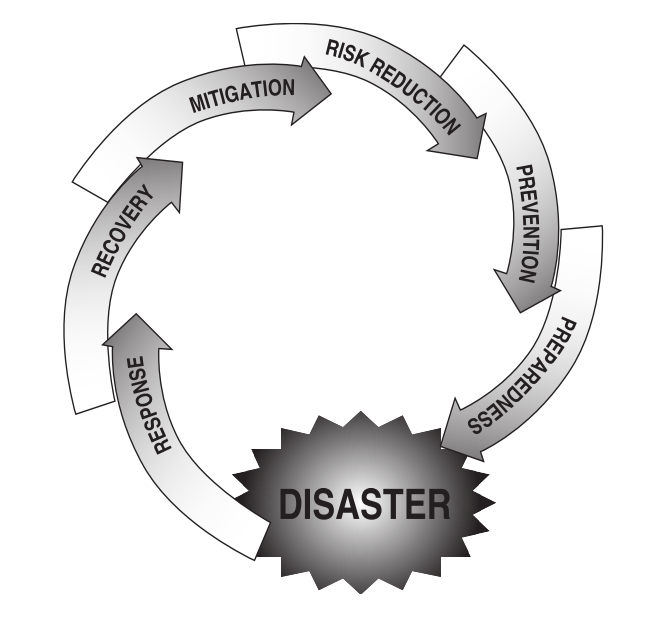
\includegraphics[width=1\textwidth]{img/background/drCircle}
  \caption{Disaster Management Circle. Credit \cite{Wattegama2012}}
  \label{fig:drCircle}
\end{figure}

\begin{enumerate}
\item Mitigation: any activity that reduces either the chance of a hazard taking place or a hazard turning into disaster.
\item Risk reduction: anticipatory measures and actions that seek to avoid future risks as a result of a disaster.
\item Prevention: avoiding a disaster even at the eleventh hour. 
\item Preparedness: plans or preparations made to save lives or property,and help the response and rescue service operations. This phase covers implementation/operation, early warning systems and capacity building so the population will react appropriately when an early warning is issued.
\item Response: includes actions taken to save lives and prevent property damage, and to preserve the environment during emergencies or disasters. The response phase is the implementation of action plans.
\item Recovery: includes actions that assist a community to return to a sense of normalcy after a disaster.
\end{enumerate}

The Disaster Response (DR) operations refer to the actions taken during or immediate aftermath of the disaster strike. In this period, a significant number of individuals may be trapped and injured. Great number of structural damages need be dealt with. Medicine, food and shelters are in great demand. This period calls for prompt action within an exceptionally short period of time \cite{Wattegama2012}. Responder team may find themselves with limited resources and need to make plans to utilities the resources in a timely and satisfactory manner \cite{Chen2005,Chen2008}. \\

%\subsection{Team coordination in disaster response}
%Malone (1990 361) defines coordination as the act of managing interdependencies between activities performed to achieve a goal. One of the very important component of coordination in DR, following sections will firstly... and then discuss how the coordination is carried out through command structure of DR team. \\

%In disaster response, team coordination is essential in order that groups of people can carry out interdependent activities together in a timely and satisfactory manner (cf. Bradshaw et al., 2011). Disaster response experts report that failures in team coordination are the most significant factor in critical emergency response (Toups et al., 2011: 2) that can cost human lives. Shared understanding, situation awareness, and alignment of cooperative action through on-going communication are key requirements to enable successful coordination. Convertino et al. (2011) design and study a set of tools to support common ground and aware- ness in emergency management. \\

\subsection{DR command structure}\label{sec:lrstructure}
The emergency response agencies typically employs a hierarchical command structure \cite{Ramchurn2015}. One widely used command and control structure the Gold, Silver, Bronze model. In this model, decision making is divided into strategic, tactical, and operational levels. The teams responsible for each are referred to as ``Gold, Silver, and Bronze'' respectively. The decisions on main objectives of the response effort are made at the strategic (Gold) level. At the tactical level, the Silver command team decides on the allocation of resources and tasks to be carried out  based on the specified objectives. At the operational level, Bronze first responders (FRs), on the ground, determine the logistics required to carry out those tasks. Information gathered from the ground is also passed back up from Bronze, through Silver, to Gold \cite{Ramchurn2015}. Some literatures \cite{Chen2005,Chen2008} also generalized the command and control structures as a generic two level model. The key characteristic of the two-level model is division between remote coordination center and on site teams.  On-site responders react to immediate scene without global picture, while the coordination center deals with strategic issues and works with a global picture, leveraging external resources to help on-site response. \\

%insert picture 

\subsection{Task planning in large scale disaster} \label{sec:LRtaskplanning}
One important characteristic of large-scale disaster is the presence of multiple spatially distributed incidents \cite{Chen2005}. To gain insight into the problem of task and resource allocation in large scale disaster, we will firstly examine how a single incident is dealt with. The procedures of dealing with single emergency incident have documented by a number of field studies \cite{Comfort2004,Dawes2004,Petrescu-prahova2005}. In Toups's \cite{Toups2011} study, fire emergency response to small-scale structural fires is depicted as follow: 

\begin{quote}
Fire emergency response is undertaken by small teams distributed throughout the incident, coordinated by an incident commander (IC) . Multiple response teams, or companies, are dispatched to any incident and cooperate around the fireground. A company officer leads each team, which consists of firefighters and/or engineers.2 Normally, each company is associated with a firefighting vehicle; an apparatus, such as an ambulance, engine, or ladder truck.\\
\end{quote}

From the depiction of single incident emergency response, we can see that a combination of different resources (e.g. ambulance, fire engine, ladder truck ) and skills (e.g. structural engineers, firefighters and medics) are deployed to the location of the incident. To deal with multiple incidents, the disaster response team has to coordinate spatially distributed resources and personnel to carry out operations (e.g. search, rescue and evacuation) \cite{Chen2005}. That is , resources and responders needed to be divided and combined in to teams and deployed to handle distributed incidents. Depending on the number of incidents, response personnel may need to dispatch, deploy and redeploy limited resources. One major concern for task planning in disaster response is how to efficiently allocate limited resources to multiple incidents with temporal and spatial constraints \cite{Bradshaw2011}.\\

Also, the task environment of DR is characterised by various uncertainties including, but not limited to hazard uncertainties, task-flow uncertainties, environmental and informational uncertainties \cite{Chen2008}. Sudden and unexpected events may occur as the disaster situation unfolds. Therefore, fixed plans of actions for responders is unlikely to work. The uncertainties may need to be handled by improvisation, prioritisation, and dynamic sourcing of capabilities \cite{Faraj2006}, which means dynamic change of plans is necessary to deal with uncertainties in dynamic task environment.\\   

In summary, responders in DR need to carry out a set of interdependent activities under time pressure and spatial constraint. Both their resource (personnel and physical assets) and capacity of problem solving required for planning may be stretched in a large-scale, multi-incident disaster. To alleviate the problem, technological support in DR has long be studied by computer scientists. We will review some of the related research areas in next section.\\


%geo-distribution and time pressure has been identified as challenges for task planning and execution. Uncertainty new means real time and dynamic task planning[chen's emergency response]. Geo distribution creates uncertain in the information [short distributed team paper][the human factor in dr paper discussion failure of communication] and creates time constraint as well because teams need to be  \\


%chen's emergency response some practitioners articles

%The fireground and surrounding space constitute a dangerous and dynamic interface ecosystem [Kerne 2005] of distributed cognition, connecting responders, victims, fire- fighting equipment, communication media, and information artifacts. Upon arriving at an incident, multiple companies distribute in and around the fireground. Compa- nies and their apparatuses are placed at strategic locations, and are moved as needed. Human operators work on and from these platforms. Firefighters and rescue workers deploy from them, taking equipment into the fireground; equipment, such as firehoses and radios, may be technologically supported by the apparatus itself (pumps and water sources, or high-power repeaters, respectively). Each apparatus, and in many cases, each human worker, is equipped with a half-duplex radio to facilitate long-range, broad- cast communication.\\

\section{Command and Control Environment}\label{sec:LRC2}
The Command-and-Control(C2) environment have been a long standing research topic in the field of HCI. The  research of C2 setting focuses on how operators manage and control safety-critical systems \cite{Fischer2015}. The studies of C2 work setting is particularly relevant to this thesis, because most emergency response operation is carried out in a C2 environment (section \ref{sec:lrstructure}). \\

In the field of CSCW, ethnographic studies are carried out to explicate work practice and organisational conduct in the C2 environment, with the aim to inform the design of technological support systems. The studies are conducted in a range of application areas such as air traffic control [-], emergency response \cite{Fischer2015} , and military operations \cite{Tolcher2005}, with the aim to provide design implications for technological support. For example, the The work of \cite{Heath1992} conducted a detailed examination of social organisation of collaborative work within a line control room in London underground. The analysis of \cite{Heath1992} particularly focus on interaction between different personnel as they coordinate a range of tasks and utilise various tools. The study revealed the methodological ways in which the participants surreptitiously monitor each other's conducts, and at the same time, render their actions visible and accountable to the other team members. Therefore, it is critical for computational systems to facilitate individuals mutually to monitor their co-participants \cite{Heath1992}.\\

Similar C2 setting can also be found in the orchestration of Mixed Reality Game(MRG) experiences in which online players in the control room and field players `on the ground' interacts through pervasive technologies such as smart phones, GPS and other mobile sensors (for details of MRG, see section x). The ethnographic studies of MRGs \cite{Benford2006}, \cite{Crabtree2004}, \cite{Koleva2001} focus the distributed natural of C2 environment. The observations in the studies reveal methodological ways in which players collectively battle the uncertainties and interruptions of technologies through distributed orchestration process. The results of the studies leads to a set of design implications for handling uncertainties and interruptions in the distributed C2 environments. \\

Apart from ethnographic studies, the impact of technology support in the control room is also assessed by human factor researchers through quantitative evaluation of operators' performance \cite{Grootjen2007}, \cite{Sharples2011}. For example, the study by \cite{Sharples2011} is conducted to assess impact of recent automation in rail way signalling operations. The studies evaluated changes of operators' performance through statistical test and quantitative comparison of observational data. The results indicate that automation is effective at reducing high level of interaction and workload. However, operators do seem to struggle to maintain awareness of system state and that they are also unable to monitor the way in which automated support makes decisions in real time. \\

While both qualitative and quantitative studies contribute to understanding of human-system interactions in complex C2 settings, this PhD work is primarily interested in understanding of social organisations of work, and follow the tradition of empirical CSCW studies to unpack the social interactions in C2 setting. \\

%The analysis is no longer primarily concerned with the individual and the system, but rather the  The ability to coordinate activities, and the process of interpretation and perception it entails, inevitably relies upon a social organisation; a body of skills and practices which allows different personnel to recognise what each other is doing and thereby produce appropriate conduct. Heath and Luff's study of London Underground shows for example how co-orientation among operators is critical in this ``multimedia environment''.\\


\section{Technological Practices in Disaster Response} \label{sec:LRApplicationAreas}
So far, we have framed the problem of task planning in DR in section \ref{sec:lrplanning} and reviewed three research domains related to development of DR planning system in this section. To give an overview of current technological practices related to planning support, This section will reviews three related research domains in the context of computational DR support, that is - GIS-based task planning systems for plan formulation and evaluation ; the Information and communication technologies (ICT) for information acquisition and management; and the AI(Artificial intelligence) based technologies for disaster simulation, and plan optimisation.  \\

This PhD work is primarily interested in a real-time task planning system that utilise ICT technologies as its underlying infrastructures and apply intelligent coordination algorithms for plan generation. This kind of system can be located in the overlapping area of the three research domains that is reviewed in this section (see figure \ref{fig:SystemFraming}).\\

\begin{figure}[h]
  \centering
  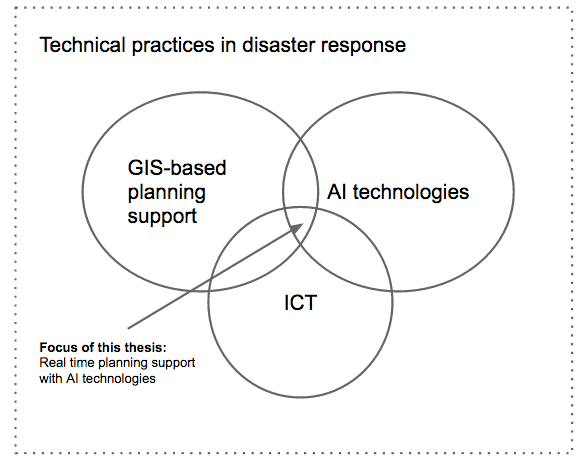
\includegraphics[width=1\textwidth]{img/background/SystemFraming}
  \caption{technological support for disaster response}
  \label{fig:SystemFraming}
\end{figure} 

\subsection{GIS-based planning support systems}
The Planning Support System (PSS) can be defined as a suite of computational components that help planners to explore and manage planning activities \cite{Geertman2004}.Literatures have documented a variety of planning support systems with a range of purposes such as land development \cite{Pettit2003}  and logistic scheduling \cite{Miller}. In the context of disaster response, planning activities  typically concern dispatch, routing and deployment of rescue resources (see section \ref{sec:LRtaskplanning}), which means the geo-information tools/systems (GIS) for spatial analysis may be a central component of a planning support suite. Therefore, this section will focus on reviewing the GIS-based PPS. \\

While the general-purpose GIS  are only designed to handle geo-spatial data \cite{Geertman2004}, the PPS may have a wide variety of functionalities to support multiple aspects of planning process, which may include, but not limited to problem diagnosis, data collection, mining and extraction, data modelling, visualisation and display, scenario-building and projection, plan formulation and evaluation, and collaborative decision-making support \cite{Geertman2004,Zerger2003}. A range of the GIS-enabled planning systems have been developed for various purposes such as  vulnerability assessment, risk management and hazard mitigation \cite{Cova199,Schooley2010}. One example is the ``Intergraph'' developed by Victorian Emergency Services (Australia) \cite{IntergraphCorporation2000}to support emergency dispatch services (e.g. ambulance, police and fire services). The system support daily response activities by providing automated geo-referencing, routing, mapping, planning and analysis \cite{Zerger2003}. Another example of GIS-based planning support is an evacuation planning tool for radiological disasters developed by \cite{Eglese1994}. The system combines simulation models and  GIS software to model evacuation routes for evacuation in radiological incidents.  It uses the spatial data structure and programmed simulation models to predict traffic flow through the road network under scenarios such as vehicle breakdowns and road closures. The system is designed for evaluation of evacuation strategies prior to disaster. Real-time decision support is not possible because the simulation is computationally intensive.\\

The `real time' task planning in DR is different from other long-term planning scenarios due to time pressure and uncertainties involved.  Responders in DR have to plan dynamically according to the disaster environment that are always quickly changing. The study of \cite{Zerger2003} have pointed some technical and social impediments for applying GIS tools to support `real-time' planning activities in DR. First, some spatial modelling and simulation technologies can be very (such as \cite{Eglese1994} ) computational intensive which makes it unable to provide results in real-time. Second, some of the planning systems are adapted from GIS software, which require high level of training to operate. Third, there are lack of social and organisational considerations in the most of existing GIS tools. For example, some PPS are based on a single computer terminal, which is unable to facilitate information sharing with multiple users in control room and `on the ground'. \\

The third point is aligned with the studies of command and control (C2) task environment (in section \ref{sec:LRC2}). The C2 environment is collaborative setting which involves complicated social interaction and organisational conducts. Therefore, the PPS designed for C2 environment should consider supporting the social conducts of responder teams. Further, the computational support in modern C2 environment (e.g. air traffic control \cite{Mercer2014} and underground control \cite{Sharples2011}) supports a range of activities such as information acquisition, analysis, decision selection and action implementation. Similar to other C2 environments, plan generation and action implementation in DR are typically fast pace and happens in parallel. The existing PPS such as \cite{IntergraphCorporation2000}, \cite{Eglese1994} only provide isolated functionalities for supporting plan generation. To realize `real-time' planning support, the author believes the PPS should be further extended or integrated with other system functionalities for action implementation, such as progress monitoring, conflict detection, and communication support.\\

%Efforts have been made to study and design such real-time task planning system for DR Wagner et al. [2004]; not Okaya et al. [2014], but the real deployments are still rare.[Bring up the previous ] Once we extend the capabilities planning system with real-time capabilities, the boundary between planning system and command/control systems (e.g ground traffic and aviation control \cite{Sharples2011}) are blurred. In this PhD work, we will call the system sitting in the middle ground area `real time planning' system. Some researches treat command and control system as tools to automate some aspects of command control activities including information acquisition, analysis, decision selection and action implementation \cite{Sharples2011}.  In contrast, a `real-time planning support system' may have stronger focus on supporting real-time plan generation and selection.

\subsection{ICT support for disaster response}
The information and communication technology support (ICT) includes communication infrastructures and software system on top of the infrastructures. The communication infrastructures refer to communication channels such as radio, television, satellite, internet, text and voice communication over mobile phone. The basic communication infrastructures have long be utilised by responders to capture both soft data (generated by human) and hard data (from sensors) for their decision making \cite{Fischer2012}. Apart from the infrastructures, the ICT software systems are playing increasingly important role. Now days, most DR practice may consists  of both the manual processes which directly relies on ICT infrastructures and the automated (or partially) process of data analysis and information management that are supported by ICT softwares. For example, the figure \ref{fig:ICTExample} illustrate a tsunami response system operated by Asian Disaster Preparedness Center(ADPC)[]. In this system,  the technical components are comprised of a network of seismographic stations, sea-level gauges and deep-sea pressure sensors. A tsunami forecasting centre is equipped with seismic processing and modelling software.  Tsunami warnings are disseminated through the communication links between national centres and the people at risk, the links include, email, television, radio, cellphones and satellites. Another scenario for ICT support can be found in most modern emergency response rooms (ERR). For instance, the ERRs in Amsterdam uses a ICT software called GMS (integrated emergency response room system) \cite{Boersma2009}. GMS is used to connect the different information sources (e.g. a national digital radio network for public safety). However, the ERRs in Amsterdam is not co-located, but divided by regions and functions (Fire,Police and Medical). GMS used by ERRs are not connected and they are tailored differently to the various needs and requests of operators. As the ERR systems are disconnected, information exchange between ERRs is conducted manually through telephones \cite{Boersma2009}.\\

\begin{figure}[h]
  \centering
  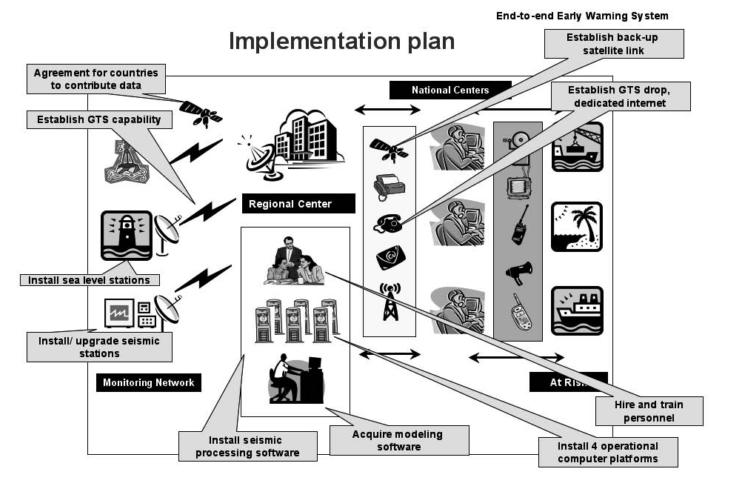
\includegraphics[width=1\textwidth]{img/background/ICTExample}
  \caption{Tsunami response system}
  \label{fig:ICTExample}
\end{figure}

With proliferation of smart phones and ubiquitous computing technologies, internet have become increasingly important in the disaster response. Web-based applications have been used in the indian ocean tsunami for tracking missing people, coordinating donors, and recording locations of shelters \cite{Wattegama2012}. The internet also expanded the possibilities for public participation. For example, the use of microblogging tools such as `tweeter' in DR have have been a popular research topic in the field of crisis informatics \cite{Kogan2012,Sarcevic2012,Starbird2010}.  The microblogging tools enabled the public to take not only a more active part in seeking information, but also in providing information to each other, as well as to formal response efforts. Crowedsourcing platform such as Ushiadidi[] is another example of ICT support for public participation in DR. The Ushiadidi platform have been used in the Haiti earthquake as a volunteer effort to produce a crisis mashup. Information about the humanitarian crisis and the response that followed was aggregated in near real time by volunteers from a variety of sources including: SMS, Web, Email, Radio, Phone, Twitter, Facebook, Television, List-serves, Live streams, Situation Reports \cite{Morrow2011}. Similarly, crowedsourced map systems such as OpenStreetMap \cite{Palen2015} have been applied in disasters (Haiti earthquake, Typhoon Yolanda) for volunteers to create updated crisis map. Although public participantion has played an important role in DR, its integration with formal response efforts is still a challenge for ICT researcher\cite{Palen2007}, and a lot of research efforts have been made to address social, organisational and technical challenges of the integration \cite{Dashti2014}, \cite{Sutton2008}.   \\

In summary, ICT infrastruce and software are commonly used in disaster response. Two case studies (tsunami response system and emergency response room support) are used to illustrate the ICT supported DR processes. Public participation is another trend of ICT system support raise from increased global access to internet. However, studies showed integration of public participation and formal response efforts is still problematic and require further research. From the author's point of view, a task planning support may heavily rely on ICT infrastructure for data acquisition and plan implementation. Functionalities of ICT software also have many overlaps with that of task planning systems, in the sense that they all support responders to acquire, process and manage information for the use of decision making in DR. \\


\subsection{Application of AI technologies}\label{sec:lraisupport}
In the field of AI, machine learning, optimisation and agent-based simulation algorithms have increased in availability for disaster response. \\

Disaster simulation technologies \cite{Okaya,Scerri2005} have long been applied in various types of disasters such as fire \cite{Tang2012}, hurricane \cite{Vickery2009} and earthquake\cite{Sobhaninejad2011} to understand the process and impact of disasters. The state of art simulation technologies are able to provide real time simulations with high data resolution. For example, the simulation platform devised by \cite{Sobhaninejad2011} is able to provide real-time simulation of ground motion and structural damage after earthquake, in an urban area with 10 4 6 structures. \\

Evacuation simulation is also extensively studied in the literatures. For example, \cite{Pillac2015} developed a simulation algorithm for large scale flood evacuation. The algorithm consider the dynamics of the flood and the state of the transportation network over time. The experiment showed this algorithm is able to provide plans to evacuate about 70,000 people in a impact region in real time.  Another example can be simulation of indoor fire evacuation devised by \cite{Tang2012}.  The algorithm combines modelling of building geometry, human behaviour, fire field to provide intelligent decision support. While results of evacuation simulations are promising in lab experiments, some studies pointed out the simulation technologies over simplified the human behaviours \cite{Hentenryck2011}. For instance, in some countries, most people disregard evacuation orders. The complexity of human behaviour raise from cultural, political, psychological factors, which makes behaviour modelling a challenging topic for AI community \cite{Provitolo2011} . \\

%Apart form disaster simulations, optimisation algorithms have been studied for resource allocation in DR [][]. The model use detailed descriptions of operational areas such as xxx,xxx,xxx and available resources to caculate the resource performance and efficiency for different tasks related to the response. It is important to deliver water, food, medicine, and other commodities .\cite{Fiedrich2000} ties as quickly as possible after a disaster strikes. For a partic- ular commodity (or collection of commodities), the problem consists in deciding 1. where to store the supply and in how much quantity; 2. how to deliver the commodity as far as possible. The first question is strategic or tactical in nature; the second one addresses the response. The overall problem is stochastic and the goal is to minimize a lexicographic objective function consisting of minimizing the unsatisfied demand, the latest delivery time, and the storage costs, using eith stochastic or robust optimization. The second objective, which is unconventional, was a DHS requirements and differs from traditional objective functions in vehicle routing which often aim at minimizing travel distance or cost. \\

Agent-based optimisation algorithm for multi-agent teams coordination is also an active research area in AI community. The coordination challenges in the time critical task environment inspired the multi-agent researchers to investigate real-time algorithms that provide optimal or near optimal task plans that can be used to guide distributed human or robotic teams \cite{Kitano2000}. Various algorithms have been designed to meet different requirements of team coordination. For example, the \cite{Lagoudakis2005} provide a number of auction-based algorithm that allocate agents to tasks considering the best routes for each agents in the team. On the other hand, \cite{Scerri2005a} devised algorithms to allocate tasks based on token passing. Their algorithms focus on matchings of task and team capabilities, which ensures that the right agents are routed to the right tasks based on capability thresholds. Other algorithms \cite{Ramchurn2010,Koes2005} also consider multiple criteria including task workload, deadline and team coalition effects. From HCI perspective, these capabilities of these algorithms are also limited by a number of factors. First, the concerns about oversimplified human behaviour modelling is applied \cite{Drury2009}. Second, because the algorithms are designed to deal with specified requirements (e.g. routing, task/skill matching) with simplified model of environments, they may be insufficient to deal with contingencies raised from messy real disaster environment \cite{Armenakis2012}.\\

It is observed that most intelligent algorithms are only studied and evaluated in the research lab. Integration of the algorithms and actual DR practices is still a multi-disciplinary research challenge. Nowdays, with the increase in the networked computers, sensors and amount of data generated from different sources in real time \cite{Ramchurn2015}, there are increasing demand for intelligent computational support of data processing and task planning. As a case study, researchers from ORCHID project have developed a prototype system - HAC-ER (Human Agent Collectives for Emergence Response) \cite{Jennings2014,Ramchurn2015,Ramchurn2015a}, which demonstrates how the AI algorithms may transform the landscape of real time task planning in DR.\\

The HAC-ER system consists of a set of connected components for real-time task planning support, each of which are powered by multiple machine learning and agent-based algorithms. First, a component called Crowedscanner is used to deal with vast quantities of unstructured data produced very rapidly on the internet as disaster unfolds, such as text messages or photographs from web-based platforms such as Twitter and Ushahidi[]. The approach is to use a machine learning algorithms (for details, see IBCC \cite{Simpson}) to fuses heterogeneous reports from both unreliable and trusted sources into a common picture of the disaster, or a heatmap of incidents. Second, multiple  UAVs (Unmanned Aerial Vehicles) is deployed as mobile sensors to search or further inspect incidents reported by crowdscanner. The control of multiple UAVs is assisted by multi-agent coordination algorithm (Max-sum \cite{Ramchurn2010}). The algorithm is capable of quickly optimise the task allocation for UAVs to visit points of interest or conduct search in an area.  Finally, responders and assets on the ground will need to be dispatched and deployed to deal with distributed incidents. Another HAC-ER component is designed to assist human operators in the control room to conduct real-time planning. The component is powered by a coordination algorithm based on MMDP modelling techniques \cite{Wu2015}, which takes into to account the priorities of incidents, and locations of responders teams and incidents. The algorithm can produces computationally optimised task allocations for responder teams to attend as many incidents as possible with a time constraint. Further, algorithms and interfaces of all components in HAC-ER are designed in a way that accept input form human operators. The HAC-ER depicted a picture in which human operators and intelligent components collaboratively conduct task planning, and the picture demonstrates the potential for applying AI in DR task planning.\\

\subsection{Summary}
This section have reviewed technological practices related to planning support in disaster response. First, there are great many GIS-enabled planning support systems (PSS). However impediments for applying the GIS-based are also identified in literatures. For example, GIS planning system with real-time capabilities are rare and there is also lack of social and organisational consideration in the design of GIS planning systems. Second, the ICT infrastructures and softwares have long be utilised by responders for managing communication and information. The author believe ICT provides the basis for real-time task in the sense that it provide functionalities to support information acquisition and management. Finally, AI researcher have devised some machine learning and agent-based algorithms to support task planning. Prototype systems have been built to demonstrate the potential for planning support based on AI technologies.\\ 

In the overlapping area of the three application domains, there is an opportunity space for real time task planning support in DR domain. The planning support system can utilise ICT technologies as its underlying infrastructures and apply intelligent coordination algorithms for plan generation. However, the literatures for building such a system are still rare, leaving a gap in literatures. This thesis is aimed to bridge the gap by studying the design and development of such DR planning support system.\\

\section{Summary}
Relevant literatures have been reviewed in this chapter. The studies of disaster response operations showed that the task planning activities is challenging due to time, spatial constraints and uncertainties in dynamically changing disaster environment. Further, the DR planning process is typically embedded in a command and control (C2) task environment. The literatures have revealed that the C2 setting is characterised by complex social interaction and organisational conducts. Therefore, technology support do not only need to provide the solution of complex coordination problems, but also need to support social aspects of planning generation in complex C2 setting. \\

There are various existing technology support designed for DR. First, the GIS-based planning support GIS functionalities with environmental modelling techniques to provide decision support for various purposes such as floor and indoor fire evacuation. However impediments for applying the GIS-based are also identified in literatures. For example, most GIS planning system can not support real time decision making and there is also lack of social and organisational consideration in the system design. Second, the ICT support system historically played an important role in DR. Now days, the ICT infrastructures and software are becoming increasingly connected at global scale, which changes the landscape of DR by expanding the possibilities of public participation. Further, the AI community have also devised various machine learning and optimization technologies for DR operations. Particularly, a number the multi-agent coordination algorithm have been devised to provide solutions on task allocations in DR. In the overlapping area of the three application domains, there is opportunity space for real time task planning support in DR domain. While the The planning support system can utilise ICT technologies as its underlying infrastructures and apply multi-agent coordination algorithms for plan generation. However, the researches for building such a system are still rare, leaving a gap in literatures.\\

\chapter{Interaction between Human and Planning support system}

Applying task planning to support complex disaster response operations may not be a straightforward process. Some HCI literatures \cite{Ackerman2000,Bowers1994,Niazkhani2009} have shown that introducing technology system to support organisational work may be extremely difficult. Use of technologies may have unexpected negative impact on human team performance. This thesis adopted a socio-technical view towards the undesirable impact of planning support technologies on human team performance. Particularly in planning support system, the socio-technical perspective concerns with issues the emerge form the gap between the human , system problem solving, namely the divide between a situated actions of human and cognitive planning model held by system [suchman]. Meanwhile, other two HCI researcher areas are particularly concerned with human system interaction. First, the research of automation design  concerns what and how to automate a working process by using computational systems. Second, the research of human agent interaction focuses on building software agent that is capable of teamworking with human operators. This section will review the three perspectives to give an conceptual background of design challenges that we may encounter when developing DR task planning support.\\

Further, studying human system interactions in real world disaster could be very challenging because disasters conditions can not be reproduced easily. Therefore, researchers have long been using gaming as an approach for studying the impact of technology support.  The section \ref{sec:LRMRgame} reviews the strengths and weakness of using game as an approach for studying disaster work setting. \\


\section{A socio-technical perspective to technology support} \label{sec:LRSocialTechnical}

A so-called socio-technical gaps that are often found in design and development of CSCW (Computer Supported Cooperative Work). The research field of CSCW addresses how collaborative activities can be supported by means of computer systems \cite{Carstensen1999}.  CSCW goes beyond building technology itself and investigates how people work within groups and organizations and the impacts of technology on those processes. The term socio-technical systems was originally coined by Emery and Trist \cite{Ropohl1999} to describe systems that involves complex interactions between humans, machines and the environmental aspects of the work system. The implication of this definition is that both social and technical factors e.g. people, machines and context need to be considered when developing such systems. Introducing a technology support system into an organization requires the technical and social aspects to be integrated, which can be a major challenge of building CSCW systems \cite{Ackerman2000}. \\

Researchers have recognised a so called socio technical gap in many CSCW systems. It is argued that \cite{Ackerman2000}  human activities is highly flexible, nuanced, and contextualized and that computational processes and entities such as information transfer, roles, and policies need to be similarly flexible. The social-technical gap is the divide between what we know we should support socially and what we can support technically \cite{Ackerman2000}, and the gap may result in serious negative impact on human activities. \cite{Bowers1994,Abbott1994a}. Therefore, it is vital to study technology in use to understand potential tensions between technical mechanism and social life \cite{Bowers1994}.  In the context of disaster response, we believe the same is true for the application of agent-based planning support. Empirical works \cite{Petrescuprahova2005,Kopena2008,Fischer2015,Zerger2003} have revealed the complexity of social and technological processes in disaster response operations. Responders with different roles have to engage in the various interdependent activities that are distributed in both time and space (see section \ref{sec:lrplanning}). To build agent-based systems that support human team coordination, exploration of such social-technical gap and its impact can be vital. \\ 

\subsection{The socio-technical gap for planning support system}
In the context of planning support, the socio-technical gap can be specifically originated from the different ways in which human and system plan and act. The view of purposeful action is adopted by many researchers and designers of intelligent systems, serving as the model of plan and action that is embedded in lots of problem solving systems \cite{Allen1984}. On this view, plan is a prerequisite of and prescribe to action. The view of purposeful action is also embraced by behavioural science as the basis for traditional view of rational human actions. However, the view of purposeful action is challenged by recent trends in sociology, arguing that prescriptive significance of plans and intentions for action is quite vague. Rather then determining the actions, the plans only serve as resource for human's practical deliberation about action \cite{Suchman1987}.\\  

\subsubsection{Planning model embedded in problem solving systems }
% The machine planning 
% The planning model, on which most system have been build on. Plan generation, replan, 
The view of purposeful action underpins the planning model form cognitive science. The planning model is embedded many of problem solving systems \cite{Suchman1987}. The model treats a plan as a sequence of actions to achieve an end goal. In problem solving systems, actions are described by prerequisites(The condition triggers action), effects (The condition after action) , and decomposition(Executing subactions) \cite{Allen1984}. The situation of action is the conditions that hinders the actors' movement to the end goal status. Some problem solving systems is only designed for plan generation. When a plan is constructed, the problem solves finished their work, assuming nothing will go wrong. However, contingent situations (or unanticipated conditions) will emerge, requiring  \cite{Suchman1987} replanning. Therefore, modern antonymous systems is typically designed to conduct planning and execution monitoring, which enable them to respond to contingent situations.\\

% figure

% Plan recognition to achieve xxx.
The recent development in artificial intelligence (e.g. multi-agent systems) requires the planning model to be extended from individual agent to multi-agent situation. To achieve concerted actions in the social situation with multiple agents, the planning model seeks to attach the knowledge of other agent's plans and actions as a type of environmental condition for planning. In this way, the basic view of single, goal directed agent (e.g. BDI model of agents \cite{Georgeff1999}) is remain intact. To obtain the knowledge of other agent's plans, agents are required to conduct plan recognition in addition to planning and execution monitoring. The basic assumption of plan recognition that agents as observers take actions of each other as evidence to form hypothesis of plans that explain intentions and actions of each other.  \\

The planning model is problematic when it is applied as model of human's ``psychological process'' of action. Studies have pointed out in many occasions human actions do not appear to follow logical steps or rational plans \cite{Suchman1987}. Researchers of cognitive science argued that the issue is due to actions under vague intents and incomplete plans. As a result, the human planning activity is often inferior version of scientific planning that need to be supported. However, many sociologists challenge the view by refuting the significance of plans in determining actions  \cite{Suchman1987}. The key argument arguing that the human action is essentially situated, not planned. This argument will be detailed in next section.\\ 

\subsubsection{Situated actions of humans}
% The human planning
% Situated actions, suchman argued it is what human follows
% Plan is just a representation of situated actions, and why it is always mistakenly treated as rational. 
In contrast to problem solving systems, recent efforts in sociology argue that human perform in . The argument adopts the view of situated action as oppose to the view of purposeful action held by AI researchers \cite{Suchman1987}. The starting point of argument is that the plan does not prescribe the actions. The plans are part of a large context of circumstance of ongoing actions, serving as a resource for deliberation on actions [ibid].\\

In the view of situated action, the plans are only representations of our actions in the form of imagined projection and recollected reconstructions, which does not have causal relation to the actions we take. Psychologists \cite{Mead1934} suggested, although a great deal of deliberation, discussion can be taken into the plan, our plans can stop short of our actual actions. And our post hoc analysis of situated actions often make it appears to have followed rational plans. \\

In contrast to plan recognition, mutual intelligibility in a social situation is not achieved by using logical formulae and formal algorithms based on behavioural observation. Instead, situated actions are highly dependent on specific occasions circumstances and social situations. Mutual intelligibility is sustained through every instance of interaction, rather than fixed social rules and constraints \cite{Suchman1987}.\\

% Situation is achieved 

\subsection{Summary}
The great divide between planning model embedded in many problem solving systems, and situated actions performed by humans signifies the issues of human system interaction in complex socio-technical systems such as disaster response management (Table \ref{tab:planningcontrast}). In contrast to fully autonomous system, computational support system have to interact with human to achieve mutual intelligibility and concerted actions. It is important to recognise the common sense planning activities of human is not a inadequate version of scientific planning model that need to be improved or supported by systems. Instead, human plans and acts in a way that is fundamentally different from machine problem solving. Therefore, a big challenge in designing technology support is how to bridge the socio-technical gap between situated action and scientific planning model.\\

\begin{table}[h]
\centering
\footnotesize

\label{my-label}
\begin{tabular}{l|ll}
                 & Plan                                                                                                                           & Interaction                                                                                                                                                                                               \\ \hline
Planning model   & \begin{tabular}[c]{@{}l@{}}Prerequisite of to and \\ prescribe to actions.\end{tabular}                                        & \begin{tabular}[c]{@{}l@{}}Shared understanding is achieved \\ through plan recoginition.\\ Plan recgnition is achieved by \\ logical formelae based on \\ observations of other's behaviour\end{tabular} \\
Situated actions & \begin{tabular}[c]{@{}l@{}}Do not prescribe actions.\\ Resource of deliberation \\ and Representation of actions.\end{tabular} & \begin{tabular}[c]{@{}l@{}}Mutual intelligently is achieved\\  through interactions embedded\\  in the social situations.\end{tabular}                                                                   
\end{tabular}
\caption{Planning model and situated action}
\label{tab:planningcontrast}
\end{table}
 
% (status of plan) The plan is essentially the simulation of actions

% Situated actions of human is inadaquate version of scientific plannning

% The gap  
% a table for contrasting 
% System is ok to follow, achieve a goal through comprehaisve search of solution space. It would be ok for fully autonmous. When in the situation of social technical system 

%For the purpose of designing usable and useful computer systems for cooperative work settings we need to know what makes work situations complex to competent actors and how computer systems may be of assistance to reduce or otherwise cope with this complexity. 

% Instructions 
% Human to Human
% Expert system


\section{Other perspectives of human system interaction}
Two HCI research areas, namely Automation design and Human agent interaction, are relevant to development of autonomous systems that collaborate with human. This section reviews literatures in these two areas, with the aim to further develop understanding of issues and challenges of human system interaction. \\


\subsection{Automation and its impact on human performance}
The aim of an automated support system is to replace the tasks originally performed by human with a machine. \cite{Bradshaw2011} . It can be defined as the execution by machine, usually computer, of a function previously performed by human \cite{Parasuraman1997}. The tasks that can be automated is used to be limited by technical capabilities, but this is no longer the case. With quick growth of machine's speed and intelligence, the tasks that can be automated is rapidly increasing, including complex cognitive activities such as information analysis, planning and decision making \cite{Parasuraman2000}. The boundary between human machine capabilities has blurred. The automation designers have to make hard choice about what to automate and to what extent.\\

One traditional approach for automation design is to simply automate all system functions that can be automated easily in a cost-effective way, leaving the all remaining tasks to human operators. The main considerations in this approach are technical capability and cost. The assumption of this approach is that the automation of sub systems functions can lead to optimisation of whole system with no detrimental impact results from the automation. However this is not always the case, Large body of empirical work in automation design \cite{Manzey2012,Parasuraman2000} have shown that the benefits of automation may not always be realized but can be offset by some unwanted performance consequences resulting from an inappropriate use of the systems. These performance consequences include overreliance on automation, loss of situation awareness, and possible loss of skills needed to perform the automated functions manually in case of automation failure \cite{Kaber1997}.\\ 

The recognition of negative automation impact leads to the challenge of interaction design for automated support.  Some researchers suggested to achieve division of labour between human and automation according to their strength and weakness. As in Fitts list \cite{Fitts} , a set of strengths and weaknesses of humans and machines is identified. On the other hand, the un-Fitts list \cite{Hoffman2002} is also proposed as alternative approach to view human-automation relationship. The approach suggest automation should be aimed to leverage and extent , rhuman capability, rather then replacing. Some study pointed out the division of labour would not be as simple as a labour division according to strength and weakness \cite{Bradshaw2011}. By delegating the same task to machine, the nature of human tasks can be changed as well. Large body of work has shown clearly that automation does not simply supplant human activity but rather changes it, often in a way that is unanticipated by the system designer \cite{Bradshaw2011}. While both Fitts and un-fitts list are useful as high-level guidelines for interaction design, the author believe it is important for system designers to study the current work settings and technologies in use, in order to gain insight into how the division of labour is naturally achieved \cite{Crabtree2012}, so that the detailed design implications could be drawn from the insights of naturally occurring labour of labour. \\


\subsubsection{The Level of Automation}\label{sec:lrloa}
Various framework models has be proposed to guide the research on automation-induced performance consequences. The framework models allow for a standardized characterization of automated systems with regards to how functions are distributed between humans and machine. One commonly recognised model is known as the Level model of Automation (LoA). Most tasks can be fully or partially automated, which implies that automation is not all or none, but can vary across a continuum of level \cite{Wickens2010}. At the lowest level, all system functions are performed manually by human operators.  At highest level, system are fully automated, taking over all system functions. In between this two extremes, there are 10 different levels of automation proposed by \cite{Wickens2010}. \\

The LoA model can be combined with more detailed classification of automation types \cite{Parasuraman2000}, \cite{Manzey2012}. In this classification,  the human information processing work is divided into four stages, which can be supported by automation individually. The four successive stages are referred to as information acquisition, information analysis, decision selection, and action execution. Each of these identified stages can be automated with a certain degree of automation. With respect to human performance consequences, it is generally assumed that higher level of automation will benefit the system by reducing workload of human operators. In contrast, it is also assumed that medium LoA can keep human in-the-loop, which in turn, prevent what has been referred to as out-of-the-loop unfamiliarity, that is, a loss of situation awareness and a loss of manual skills \cite{Kaber1997},\cite{Parasuraman2010}.\\

While the model has been commonly adopted in to study the one-to-one operator-system interaction (e.g. autopilots[], tele-oporation \cite{Schwarz2014}), the author believe that the model may be insufficient to capture complexity of the interactions in the context of technology support for organisational work. For example, automation of a single function may have implications on roles and responsibility of many participants in the system and fundamentally change social conducts within an organisation. However, despite its drawbacks, some concepts and vocabularies in the LoA model are adopted by this research to characterise the possible types and levels of the automated planning support and their implications on interaction designs (detailed in section x).\\

%which keeps the human in the loop at least to some extent, has been assumed to provide the best choice for realizing benefits from automation and, at the same time, preventing  namely, a loss of situation awareness and a loss of manual skills, which may lead to performance problems if the operator has to resume manual control after an automation breakdown (Endsley & Kiris, 1995).%One of the currently most recognized models in this respect is the types and levels taxonomy of automation proposed by  et al. (2000). This model distinguishes automated systems with respect to two aspects. The first aspect involves the stages of human information processing that are supported by a given automated system. Four successive stages are distinguished, which are referred to as information acquisition, information analysis, decision making and response selection, and action execution. The Wickens, Li, Santamaria, Sebok, and Sarter (2010). According to this concept, “higher degrees of automation can be accomplished by both higher levels within a stage and by including later stages” (Wickens et al., 2010, p. 389). For example, More recently, another alternative model of automation to guide automation design is proposed Most tasks can be fully or partially automated, which implies that automation is not all or none, but can vary across a continuum of level []. At the lowest level, all system functions are performed manually by human operators.  At highest level, system are fully automated, taking over all system functions. In between this two extremes, 10 different levels of automation are proposed by xxx. As shown in table x. 

\subsection{Human Agent Interactions}\ref{sec:LRHAI}
Human agent interactions (HAI) is a research area that has strong overlapping with automation design, in that they both concerned with the impact of automation (i.e. computational systems) on human performance. While automation design is trying to answer the question of what and to what extent the automation should be, the study of human agent interaction concerns the issues of interaction design related to development of human agent system, with the aim to develop agents which is good at teamworking with human operators \cite{Bradshaw2011},\cite{Sukthankara}. \\

The term ``software agent'' is commonly defined as the software that can operate independently without constant human supervision\cite{Vlassis2007}. The agent researchers investigate infrastructure, language and communication to realize coordinated agent software system \cite{Nwana1996}. More recently, the use of the word software agent become much more diversified, as agent researchers has made attempts to investigate broader wide range of classes and types of agents such as interface agent, collaborative agent and information agent \cite{Nwana1996}.  \\

Some HAI researchers adopted a view that human and agents are equally important team players in a human agent system \cite{Sukthankara}. It highlights the importance of mutual interaction between human and agents that can enhance the competencies of both human and systems. From this perspective, the aim of automation is no longer "replace" human but achieve an human-machine symbiosis through effective human agent coordination. As researchers realize the effective human-machine symbiosis requires sophisticated interactions design between human and agent, the ``social'' issues of automation is thought to be as important as technical issues\cite{Bradshaw2011}. To build socially acceptable agent systems, research communities have formed around the topics of interface agents and assistants, adjustable autonomy and mixed-initiative interactions. The following sections review the literatures of the three HAI research topics, to overview the state of art techniques of building teamwork agent. 

\subsubsection{Interface Agents and Assistants}
An interface agent is the software that actively assists a user in operating an interactive interface \cite{Lieberman2003}. The metaphor of personal assistant is used to design the interaction between human and the agent. The software behave like a personal assistant who is collaborating with the user in the same work environment \cite{Lieberman1997}. Opposed to a direction manipulation interface, the assistant learns the user's goal, interests, habits and preferences (as well as those of his or her community) by observing user's actions and behaviours,  so that it can effectively provide suggestions or directly take interface actions to support human performing tasks \cite{Maes1994}.\\

User modelling is a typical approach for implementing interface agents. The user model is the program's expectation of what a user will do, what they need to be told and how they will respond \cite{Lieberman2003}.  The most sophisticated way to acquire user models are adaptive, which means they can create dynamic behaviour without being pre-programmed. For example, the user interface could learn common misspellings and typos and remind a user of how to correct them \cite{Lieberman2003}.\\

The user modelling approach has been adopted to build various agent systems. For example, Maxims \cite{Metral1998} is an agent that assists the user to organise their emails. Maxims learns to prioritize, delete, forward, sort and archive mail messages on behalf of the user. The agent continuously learns the user as the user deals with emails. The user modelling technique is also applied to implement a meeting scheduling agent \cite{Kozierok1993}. The agent assists a user with the scheduling of meetings (accept/reject, schedule, reschedule, negotiate meeting times, etc.) based on continuous learning of user's preference. Other examples applications ranges from new filtering, music/book recommendation \cite{Lieberman2003} to smart home control \cite{Costanza2014}.



%An interface agent can observe actions taken by the user in a direct manipulation interface, can sense the objects that the user sees on the screen, and can itself take actions by invoking the commands provided by the interface. The agent can add graphics or animation to the interface, it can use speech input or output, or communicate via other sensory streams. Increasingly, agents also will use sensors and effectors that sense and act directly with the real world. An agent that senses force in an exercise machine or moves a bulldozer blade can also be an interface agent. \

%The software is designed with the methpor of personal assistance. Some of them do reasoning and inference, and some of them have domain-specific knowledge or procedures that enable them to perform useful tasks. Some of them learn through interaction with their users and adapt to context.

%Every computer program has a user model, even if only implicitly. The user model is the program’s expectation of what a user will do, what they need to be told and how they will respond. Historically, it is hard-wired into the program. Command-line interfaces are predicated on the unrealistic assumption that the user knows all commands and can type them in without spelling or punctuation errors. This implicit model of the user interface coexists with a model of the task and domain. In more sophisticated user interface agents, it is often useful to be make the model more explicit so it can be manipulated and reasoned about. Interface agents may also need to move from the static, implicit models found in conventional programs, to more explicit and dynamic models. In a dynamic user model, the system could notice that the user is using a new feature that he or she never has before, and offer tutorial information. The most sophisticated way to acquire user models are adaptive, which means they can create dynamic behavior without being pre-programmed. The user interface could learn common misspellings and typos and remind a user of how to correct them. The interface could offer syntactic or presentation alternatives. The interface could watch user performance and suggest ways in which it might be improved. The simplest way for an agent to construct a user model is to have explicit interaction with the user. If the user accepts suggestions from the computer such as corrections to misspelled words, those could be added to a user model. More interesting is when the user model is constructed implicitly, by the computer making observations about user behavior that can be used to improve subsequent performance. For example, the user habitually drops an item close to a window instead of in the window and then makes a correction, the computer could at some point surmise that the person’s goal is to put things into the window. The computer should either suggest it or do it for them.\\

\subsubsection{Adjustable Autonomy}
The `Adjustable  autonomy' is a concept emerged from the research of human agent teamwork. While in tradition systems, the division of labour between human and agent is pre-programmed (i.e. fixed level of autonomy),  the system with adjustable autonomy have  reasonable dynamism with a sufficiently fine-grained range of automation levels. People want to maintain that boundary of automation at a point that minimizes their need to attend to interaction with the agent while providing them with a sufficiently comfortable level of assurance that nothing will go wrong \cite{Bradshaw2003}.The concept of `adjustable autonomy' has be widely adapted to guide a wide range of areas such as tele-operation \cite{Schwarz2014}, \cite{Goodrich2001a}, smart home control \cite{Costanza2014} and the domain of space exploration  \cite{Doraisa}. \\

\subsubsection{Mixed Initiative Systems}
``Mixed initiative'' is another approach adopted by researchers to design human agent interaction.  Mixed-initiative refers to a flexible interaction strategy, where each agent can contribute to the task what it does best \cite{Allen1999}. In the most general cases, the agents' roles are not determined in advance, but opportunistically negotiated between them as the problem is being solved. At any one time, one agent might have the initiative controlling the interaction while the other works to assist it, contributing to the interaction as required \cite{Horvitz1999}.\\

Practitioners have devised algorithms, interfaces and applications that facilities ``Mixed Initiative'' planning and control \cite{Ferguson1996}, \cite{Burstein2003}, \cite{Hardin2009}, \cite{Zimmerman2007} . One example is the interactive optimisation algorithm designed by \cite{Yang2012} to support environmental planning. Problem-solving in environmental planning typically involves multiple criteria, which can be qualitative or quantitative. The Interactive algorithm (IGA) allows a human decision maker to actively participant in the optimization process, and thereby provides means to include qualitative expert knowledge within its solution space searching process.\\


\subsection{Summary}
Through reviewing HCI research from two perspectives (Automation studies and Human agent interaction), we developed the understanding of the interaction challenges raised from integrating technology with humans' working process.  First, the automation designers realised technology can bring unexpected human performance consequence. The automation designers devised LoA modal as a way to view alternative ways we can automate a process. Although there are limitations, the model still provides useful guidelines/terminologies as a starting point for designing human system interactions. Second, the researchers of human agent interaction attempted to realise human system symbiosis by developing agent software with social capabilities of teamworking with human. A number of interaction design guidelines and metaphors raised from HAI literatures such as agent assistant, adjustable autonomy and mixed initiative interaction.  \\ 


\section{Game as an approach to study human system interaction } \label{sec:LRMRgame}
This PhD work adopts serious mixed reality game approach to investigate the socio-technical surrounding agent planning support for disaster response operations. This section will firstly review the literatures of serious games to give an overview of history and applications of serious games. In section \ref{sec:LRMRgame}, mixed reality game (MRG) will be introduced, followed by discussion of the potential for using MRGs to support ethnographic study of ubiquitous systems, which underpins rationale of the serious MRG approach applied in this PhD study.\\ 


%COOP
%We adopt a serious mixed-reality games approach to create a setting in which participants experience physical exertion and stress through bodily activity and time pressure, mirroring aspects of a real disaster setting (PAHO, 2001). We use game probes as a complementary approach to gathering system requirements for real-world settings, for example in addition to co-designing with users. Our game probe explores a socio-technical setting in which field responders receive guidance from a central command headquarters (‘HQ’), inspired by the concept of the Sector Coordinator in USAR task forces (INSARAG, 2012). \\
%Computational simulations, particularly agent-based simulations of disasters, are the predominant approach in the computing literature to predict the consequences of “courses of action” (Hawe et al., 2012), e.g., to model first responder information flow (Robinson and Brown, 2005), or logistic distribution of emergency relief supplies (Lee et al., 2007). \\

%Limitations of the veracity of computational simulations are manifold. For ex-ample, Simonovic highlights that simulations may rely on unrealistic geographical topography, and most importantly, may not account for “human psychosocial characteristics and individual movement, and (…) learning ability” (Simonovic, 2009: 89). The impact of emotional and physical responses likely in a disaster, such as stress, fear, exertion or panic (Drury et al., 2009) remains underaddressed in approaches that rely purely on computational simulation. 
%One of our work’s main objectives is to study interaction and coordination sit-uated in rich and ‘messy’ real-world socio-technical settings. As it is difficult to deploy technological prototypes in real disasters, game-like simulations have been adopted to study technology interaction in disaster scenarios, for example to pre-pare first responders for scenarios in which hazardous materials are involved (Losh, 2007). Abbasi et al. (2012) present a study in which locally distributed par-ticipants played the role of victims asking for help via social media in a simulated crisis, and participants that played the role of first responders used a coordination system to filter messages and mobilize the appropriate responder teams according to their assigned capabilities. Toups, Kerne and Hamilton (2011) present the de-sign and evaluation of the Team Coordination Game, which teaches participants effective cooperation and – in particular – communication, based on a zero-fidelity simulation of team coordination that focuses on distributed cognition in lieu of concrete details, yet draws directly from fire emergency response work practice.\\

%We adopt a serious-mixed reality games approach (Fischer et al., 2012) to cre-ate a game probe that enables studying team coordination, interaction and com-munication in a real-world disaster scenario whilst providing confidence in the ef-ficacy of behavioural observations. Suspension of disbelief occurs frequently in the play of pervasive or mixed-reality games (Stenros et al., 2009). Mixed-reality games bridge the physical and the digital (Benford et al., 2005). They serve as a vehicle to study distributed interactions across multiple devices and ubiquitous computing environments ‘in the wild’ (Crabtree et al., 2006). \\
%One important characteristic of large-scale disaster is the presence of multiple spatially distributed incidents (Chen et al., 2005). To deal with multiple incidents, the disaster response team has to coordinate spatially distributed resources and personnel to carry out operations (e.g. search, rescue and evacuation). 
%Depending on the proliferation of incidents, response personnel may need to dispatch, deploy and redeploy limited resources. Coordination is required to effi-ciently allocate limited resources to multiple incidents with temporal and spatial constraints imposed by the nature of disasters. \\

%Mixed-reality games (MRG) share a common set of characteristics with time critical settings, such as disaster response (DR):
%Bridging the physical and the digital. Both DR as well as MRGs routinely bridge the physical and the digital as part of their actors’ coordination (Benford et al., 2005). DR for example makes use of the twitterverse to inform real world response (e.g., Sarcevic et al., 2012).
%Orchestration. DR and MRGs are both highly orchestrated activities. Author-ing and orchestration tools `behind the scenes' of an MRG, as well as player in-terfaces, provide managers, players and spectators with different temporal and spatial views of the game world in order to support the experience (Crabtree et al., 2004). These settings are surprisingly comparable to the `control room' of a disaster response operation, in their collections of sophisticated technological arrangements to communicate and coordinate real-time information streams, in order to create a holistic view amidst an immersive setting of interest.\\
%On-the-ground and online. In both DR, as well as in MRGs, people on the ground often work with people online to solve a common problem. Sarcevic et al. (2012) show how understanding online content can foster understanding of medical coordination challenges in DR on the ground. MRGs often leverage the fact that people on the ground and online have different views of the world, which are turned into different abilities within the game (Flintham et al., 2003).\\ 
%These key characteristics illustrate the overlap between time-critical coordina-tion in MRGs and DR. This perspective underlies our motivation to explore the approach of studying team coordination through a game probe.\\



%=========
%Computational simulations are likely to be insufficient in elucidating the social and interactional issues around agent-based coordination support [18]. Therefore we adopt a mixed-reality game approach to put people under realistic cognitive and physical stress. Mixed-reality games are recreational experiences that make use of pervasive technologies such as smart phones, wireless technologies and sensors with the aim of blending game events into a real world environment [6]. Arguably, they have become an established vehicle to explore socio-technical issues in complex real world settings [5]. The major advantage of mixed-reality games is the fact that they are situated in the real world, which arguably leads to increased efficacy of the behavioural observations when compared to computational simulations. 
%

\subsection{Serious Game}
There are various definitions for the term `serious game' in literatures. One issue that most of the literatures agreed on about `serious game' is that the term is concerned with the use of games and gaming technology for the purposes other then mere entertainment, such as education, training, healthcare, and advertisement.\cite{Susi2007} Although serious games usually have looks and feels of digital games, they are actually simulations of real-world events or processes. by engaging the participants with simulated environments and systems, the serious games allow learners to experience situations that are impossible in the real world for reasons of safety, cost, time, etc. \cite{Squire2003,Meesters2013}. Recently, the serious games have increasingly been applied in the area of disaster response. In particular, 'serious games' are developed for training and simulation of terrorist attacks, disease outbreaks, biohazards, traffic control and fire fighting etc \cite{Susi2007,Squire2003}. \\

One good example of serious game for disaster response(DR) is the ``Biohazard'' developed by MIT Comparative Media Studies \cite{Squire2003}. The video game is designed to train emergency responders to deal with toxic spills in public locations. Emergency responders work in teams to organize the response to a gas attack in a crowded suburban shopping mall. The game objective is to save as many civilians as possible under time pressure. In the game,  players need to quickly assess the situation, divide into teams, and coordinate with each other to identify source of chemical spill. Players can thus practice recognizing the signs of different chemicals and viruses, examining victims' symptoms, and observing pattern of chemicals spread in differing environmental conditions \cite{Susi2007}.\\

%insert figure

Another example of DR serious game could be the team coordination game developed by Toups, Kerne and Hamilton \cite{Toups2011}, which teaches participants effective cooperation and communication, based on a zero-fidelity simulation of team coordination that focuses on distributed cognition in lieu of concrete details, yet draws directly from fire emergency response work practice \cite{Toups2011}. User study and evaluation of the coordination game have suggested that the a serious game built with low fidelity approach can still help responders to improve their coordination skills.\\

The advantage of serious games in disaster response domain may be obvious. Creating high fidelity excises for disaster response could be costly and dangerous, while the serious games allow participants to repetitively practice without danger and high cost. For instance, the game Biohazard\cite{Susi2007} enable players to experiment with a multitude of different task conditions and strategies with simple change of some game variables.\\

However, there are also concerns that the existing serious games often fails to capture the social aspects of DR operations. For example, it is argued that the game Biohazard failed to capture complexity of victims behaviour in highly stressful, emergency situations. Therefore, the game may not be able to help responders to develop interpersonal skill (expressed through voice, gestures) which are required to deal with panicked victims \cite{Susi2007}. In fact, the serious games are usually not designed to simulate all aspects of DR operations, but only to mirror some aspects of DR practices and processes (e.g. zero fidelity coordination game). Serious games are thus not a replacement for field trials and other training methods, but a tool responders can use to explore ideas and talk about their practice.\\

%limitation. People can be unpredictable, particularly in highly stressful, emergency situations. Dealing with a panicked public demands a type of interpersonal skill expressed through voice, gestures, and demean or that contemporary game interfaces cannot capture. Despite the many advances in artificial intelligence in games, characters still can't express a full range of emotional responses in dynamic reaction to events. Clearly, Biohazard is no replacement for experience or even field trials and manuals. Rather, it is a tool that responders can use to explore ideas and talk about their practice. [paraphase] ----- people in DR can be , the game based simulation may fail to simulate panicked public demands and emotional human response. Therefore, the game may not be enough for training of  the human and social aspects of DR domain. Therefore

\subsection{Mixed Reality Games}
Mixed-reality games are one type of digital game which tries to bridge the physical and the digital \cite{Benford2005} would. The term `mixed reality' refers to virtual experiences being played out in real-world spaces. This kind of games typically use pervasive technologies, such as cellular phones, GPS, Bluetooth, wireless network and sensors, with the aim to blend virtual game events into people's life and real world environment. Some researchers have recognised the potential to adapt mixed reality games for training purposes in Disaster Response (DR) domains \cite{Fischer2012}, as the mixed reality game is thought to be a powerful way of exposing participants to learning experiences not otherwise possible. \\

Arguably, the mixed reality game is also becoming an established vehicle to study distributed interactions across multiple devices and ubiquitous computing environments `in the wild' \cite{Crabtree2006, Benford2005, Fischer2012}. The emergence of ubiquitous computing features distributed interaction across a burgeoning array of small, mobile devices and online environments. Because the mixed reality game also create such an ubiquitous computing environment,  the mixed reality game is thought to be an ideal platform for ethnographer and system designer to investigate issues of distributed interactions in the future ubiquitous computing systems.\\

Further, the literature \cite{Fischer2012} also discovered that a DR support systems potentially shares a set of characteristics with mixed reality games, which suggests mixed reality game could be a platform for investigating issues of interactions in the DR setting:\\

\begin{enumerate}
\item Bridging the physical and the digital. Both DR as well as MRGs routinely bridge the physical and the digital as part of their actors` coordination \cite{Benford2005}. DR for example makes use of the twitterverse to inform real world response (e.g., Sarcevic et al., 2012 \cite{Sarcevic2012}).

\item Orchestration. DR and MRGs are both highly orchestrated activities. Author-ing and orchestration tools `behind the scenes' of an MRG, as well as player interfaces, provide managers, players and spectators with different temporal and spatial views of the game world in order to support the experience \cite{Crabtree2004}. These settings are surprisingly comparable to the `control room' of a disaster response operation, in their collections of sophisticated technological arrangements to communicate and coordinate real-time information streams, in order to create a holistic view amidst an immersive setting of interest.\\

\item On-the-ground and online. In both DR, as well as in MRGs, people on the ground often work with people online to solve a common problem. Sarcevic et al. (2012)\cite{Sarcevic2012} show how understanding online content can foster understanding of medical coordination challenges in DR on the ground. MRGs often leverage the fact that people on the ground and online have different views of the world, which are turned into different abilities within the game \cite{Flintham2003}.\\ 

\end{enumerate}

These key characteristics illustrate the overlap between time-critical, distributed coordination in mixed reality game and DR operation, which underpins the motivation for applying the mixed reality game as the approach to investigate socio-technical involved in developing future DR support systems \cite{Fischer2012}.\\

%The emergence of ubiquitous computing raises new challenges for ethnography however, distributing interaction across a burgeoning array of small, mobile devices and online environments which exploit invisible sensing systems. Understanding interaction requires ethnographers to reconcile interactions that are, for example, distributed across devices on the street with online interactions in order to assemble coherent understandings of the social character and purchase of ubiquitous computing systems. We


%Mixed-reality games bridge the physical and the digital (Benford et al., 2005). 

%Ubiquitous gaming is one of the most exciting ideas to emerge from the games industry in recent years. Ubiquitous games can be played anytime, anywhere and often play out across multiple media. For example, Electronic Arts' Majestic uses cell phones, desktop computers, and fax machines (among other technologies) to immerse players in a multiplayer conspiracy theory game. Such games motivate players to investigate, weigh evidence, compare notes, test hypothesis, and synthesize information as they draw conclusions about what has occurred and why. We use the terms enhanced reality or augmented reality to refer to virtual experiences being played out in real-world spaces. While such game experiences may seem prohibitively expensive, recent handheld technologies, which can now combine cellular phone, GPS, Bluetooth, wireless Internet, multimedia capabilities, and infrared technologies into one machine, make such experiences possible even on the level of an individual school.\\


%*****************************************
%*****************************************
%*****************************************
%*****************************************
%*****************************************

%\section{Ethnomethodology}

%The method of observing participants in the field study is informed by Ethnomethodology (EM). Following the tradition of ethnography, EM seeks to explicate real-world organisation of works by adopting the naturalistic stance. The EM places methodological emphasis on rigorous description of the situated (i.e. local, observable) actions and practices (Suchman, 1987) in and through the contingent accomplishment of daily activities. The EM-informed ethnography arguably helps answering what might be regarded as an essential question in design: what to automate and (Crabtree et al. 3) what to leave to human skill, competence, judgement, experience and expertise. By producing description of the actions and practices in and through which the work `gets done' time and time by the members, The EM could inform the system design by uncovering what actions and activities we should therefore support.\\

%For the purpose of this thesis, the social situation the interaction with and around the planning support was argued to be a critical factor to understand how social organisation of work is achieved participants with the existence of a planning support system. Observation of the situated actions and practice employed by the participants was a key method for the field study. The use of the system was observed and filmed for later analysis. Video is widely recognised as an important resource for ethnographies around technology use (Crabtree et al., 2006). The next section will go through the method of video-based interaction analysis for unpacking the interactions observed in the field. \\

\section{Summary}


There has be a long standing tradition for HCI community to study the relationship between human and technology support. Studies in three HCI sub domains (CSCW,Automation design, and Human agent interaction (HAI)) all recognised the socio-technical challenges raised from integrating technology with humans' working process.the  The studies in this PhD work align with the tradition of empirical CSCW systems to investigate complex collaborative work in organisational setting.  On the other hand, the research of automation design developed LoA (Level of Autonomy) model to frame alternative ways we can automate a process. Although there are limitations, the model still provides useful guidelines/terminologies as a starting point for designing human system interactions. Further, the study of human agent interaction tried to tackle the interaction challenge by developing agent software with social capabilities of teamworking. Various approaches has been adopted by HAI researcher (e.g. interface agent, mixed initiative, adjustable autonomy), which can serve as guidelines for interaction design.\\

Further, study of disaster response operation is difficult due to its safety critical nature. Game approach has long been an established vehicle for behavioural studies in disaster response setting. In particular, this PhD work adopts the mixed reality gaming as the  approach to study distributed interactions across multiple devices and ubiquitous computing environments `in the wild'. \\


